\documentclass[12pt]{article}
\usepackage[top=1in,bottom=1in,left=1in,right=1in]{geometry}
\usepackage{alltt}
\usepackage{array}	
\usepackage{graphicx}
\usepackage{tabularx}
\usepackage{verbatim}
\usepackage{setspace}
\usepackage{listings}
\usepackage{amssymb,amsmath, amsthm}

\title{SOEN331: Introduction to Formal Methods\\for Software Engineering\\
Assignment 2 on Extended Finite State Machines}
\author{Martin Marcos 40041398,\\ Samantha Guillemette 26609198,\\ Deepkumar Patel 40096716  }

\date{\today}

\begin{document}
\begin{spacing}{1.5}

\maketitle

\section{Driver-less car system formal specification}

\noindent The EFSM of the driver-less car system is the tuple $S = (Q, \Sigma_1, \Sigma_2, q_0, V, \Lambda)$, where\\

\noindent $Q = \{idle, parked~mode, manual~mode, cruise~mode, marked~mode, panic~mode, exit\}$\\
\noindent $\Sigma_1 = \{start, cruise~signal, switch, arrived, unforseen,panic~off, off\}$\\
\noindent $\Sigma_2 = \{beep, hazard~off\}$\\
\noindent $q_0: idle$\\
\noindent $V: destination = \{set, no\}$\\
\noindent $\Lambda$: Transition specifications\\
\indent 1. $\rightarrow idle$\\
\indent 2. $idle \xrightarrow {\text { start }} parked mode$\\
\indent 3. $parked~mode  \xrightarrow {\text { off }} off?$\\
\indent 4. $parked~mode  \xrightarrow {\text { cruise signal [no dest] }} manual~mode$\\
\indent 5. $parked~mode  \xrightarrow {\text { cruise signal [set dest] / beep }} cruise~mode$\\
\indent 6. $manual~mode  \xrightarrow {\text { cruise signal [set dest] }} cruise~mode$\\
\indent 7. $cruise~mode  \xrightarrow {\text { switch }} manual~mode$\\
\indent 8. $cruise~mode  \xrightarrow {\text { arrived }} parked~mode$\\
\indent 9. $cruise~mode  \xrightarrow {\text { unforseen }} panic~mode$\\
\indent 10. $manual~mode  \xrightarrow {\text { stop }} marked~mode$\\
\indent 11. $panic~mode  \xrightarrow {\text { panic off / hazard off}} manual~mode$\\

\noindent The UML state diagram is shown in Figure~\ref{fig:main-system-fig}\\


\noindent As \textit{cruise} is a composite state, it is defined as the tuple $S = (Q, \Sigma_1, \Sigma_2, q_0, V, \Lambda)$, where\\

\noindent $Q = \{tailing~mode, changing~lane~mode, navigation~mode\}$\\
\noindent $\Sigma_1 = \{i~to~c, t~to~c, c~to~t, c~to~n, n~to~c\}$\\
\noindent $\Sigma_2 = $\\
\noindent $q_0: tailing~mode$\\
\noindent $V: $\\
\noindent $\Lambda$: Transition specifications\\
\indent 1. $\rightarrow tailing~mode$\\
\indent 2. $\xrightarrow {\text{i to c}} changing~lane~mode$\\
\indent 3. $tailing~mode \xrightarrow {\text { t to c }} changing~lane~mode$\\
\indent 4. $changing~lane~mode \xrightarrow {\text { c to t }} tailing~mode$\\
\indent 5. $changing~lane~mode \xrightarrow {\text { c to n }} navigation~mode$\\
\indent 6. $navigation~mode \xrightarrow {\text { n to c }} changing~lane~mode$\\

\noindent The UML state diagram is shown in Figure~\ref{fig:cruise-mode-fig}\\


\noindent As \textit{tailing} is a composite state, it is defined as the tuple $S = (Q, \Sigma_1, \Sigma_2, q_0, V, \Lambda)$, where\\

\noindent $Q = \{accelerate, decelerate, change~lane~mode\}$\\
\noindent $\Sigma_1 = \{obstacle\}$\\
\noindent $\Sigma_2 = \{t~to~c, maintain~speed, switch~lane\}$\\
\noindent $q_0: tailing~mode$\\
\noindent $V: speedOfCar : \{minSpeedRange, maxSpeedRange\},$\\
\indent $distanceOfCar, minSpeedRange, maxSpeedRange, minDistance: \mathbb{R} $\\
\noindent $\Lambda$: Transition specifications\\
\indent 1. $\xrightarrow {\text{[s\textless minSpeedRange]}} accelerate$\\
\indent 2. $\xrightarrow {\text{[maxSpeedRange \textless s\textgreater minSpeedRange]/t to c; maintain speed}} change~lane~mode$\\
\indent 3. $\xrightarrow {\text{obstacle[d\textless minDistance]/t to c; switch lane}} change~lane~mode$\\
\indent 4. $\xrightarrow {\text{[s\textgreater minSpeedRange or d\textless minDistance]}} decelerate$\\

\noindent The UML state diagram is shown in Figure~\ref{fig:tailing-mode-fig}\\


\noindent As \textit{changing lane} is a composite state, it is defined as the tuple $S = (Q, \Sigma_1, \Sigma_2, q_0, V, \Lambda)$, where\\

\noindent $Q = \{maintain~car~speed, tailing~mode, change~lane~mode, cruise~mode, panic~mode\}$\\
\noindent $\Sigma_1 = \{maintain~speed, switch~lane, cannot~change~lane\}$\\
\noindent $\Sigma_2 = \{c~to~t, panic\}$\\
\noindent $q_0: changing~lane~mode$\\
\noindent $V: targetLane: \{car~in~t, car~not~in~t\}$,\\
\indent $speedOfCar: \{minSpeedRange, maxSpeedRange\},$\\
\indent $distanceOfCar, minSpeedRange, maxSpeedRange, minDistance: \mathbb{R} $\\
\noindent $\Lambda$: Transition specifications\\
\indent 1. $\xrightarrow {\text{maintain speed [d\textgreater = minDistance]}} maintain~car~speed$\\
\indent 2. $maintain~car~speed\xrightarrow {\text{[d\textgreater = minDistance]}} maintain~car~speed$\\
\indent 3. $maintain~car~speed\xrightarrow {\text{[d\textless minDistance]/c to t}} tailing~mode$\\
\indent 4. $\xrightarrow {\text{maintain speed [d\textless minDistance]/c to t}} tailing~mode$\\
\indent 5. $\xrightarrow {\text{maintain speed [s\textgreater maxSpeedRange \& s\textless minSpeedRange]/c to t}} tailing~mode$\\
\indent 6. $\xrightarrow {\text{switch lane[car not in t]}} change~lane~mode$\\
\indent 7. $\xrightarrow {\text{switch lane[car in t]/c to n}} cruise~mode$\\
\indent 8. $\xrightarrow {\text{switch lane;cannot change lane/panic}} panic~mode$\\
\indent 9. $change~lane~mode\xrightarrow {\text{[car not in t]}} change~lane~mode$\\
\indent 10. $change~lane~mode\xrightarrow {\text{[car in t]/c to n}} cruise~mode$\\
\indent 11. $change~lane~mode\xrightarrow {\text{cannot change lane/panic}} panic~mode$\\

\noindent The UML state diagram is shown in Figure~\ref{fig:changing-lane-mode-fig}\\

\noindent As \textit{navigation} is a composite state, it is defined as the tuple $S = (Q, \Sigma_1, \Sigma_2, q_0, V, \Lambda)$, where\\

\noindent $Q = \{turn~left,turn~right, turn~left~ahead, turn~right~ahead, changing~lane~mode,destination~ahead, arrived~destination\}$\\
\noindent $\Sigma_1 = \{d~on~left, d~on~right, TLA, TRA, d~ahead, car~at~d\}$\\
\noindent $\Sigma_2 = \{turn~left, turn~right, dest~ahead, car~in~t, n~to~c, switch~lane, arrived\}$\\
\noindent $q_0: changing~lane~mode$\\
\noindent $V: targetLane: \{car~in~t, car~not~in~t\}$,\\
\noindent $\Lambda$: Transition specifications\\
\indent 1. $\xrightarrow {\text{d on left/turn left}} turn~left$\\
\indent 2. $\xrightarrow {\text{d on right/turn right}} turn~right$\\
\indent 3. $\xrightarrow {\text{TLA[car not in t]}} turn~left~ahead$\\
\indent 4. $\xrightarrow {\text{TRA[car not in t]}} turn~right~ahead$\\
\indent 5. $\xrightarrow {\text{TLA/[car not in t]}} turn~left~ahead$\\
\indent 6. $turn~left~ahead\xrightarrow {\text{/n to c; switch lane}} changing~lane~mode$\\
\indent 7. $turn~right~ahead\xrightarrow {\text{/n to c; switch lane}} changing~lane~mode$\\
\indent 8. $destination~ahead\xrightarrow {\text{car at d/arrived}} arrived~destination$\\

\noindent The UML state diagram is shown in Figure~\ref{fig:navigation-mode-fig}\\

\newpage

\section{UML state diagrams}

\begin{figure}[h!]
	\centering
		\includegraphics[width=0.8\textwidth]{./A2_Figures/4.1-Main-System.eps}
		  \caption{Main System.}
  \label{fig:main-system-fig}
\end{figure}

\begin{figure}[h!]
	\centering
		\includegraphics[width=0.8\textwidth]{./A2_Figures/A2_SOEN331_Cruise.eps}
		  \caption{Cruise Mode.}
  \label{fig:cruise-mode-fig}
\end{figure}

\begin{figure}[h!]
	\centering
		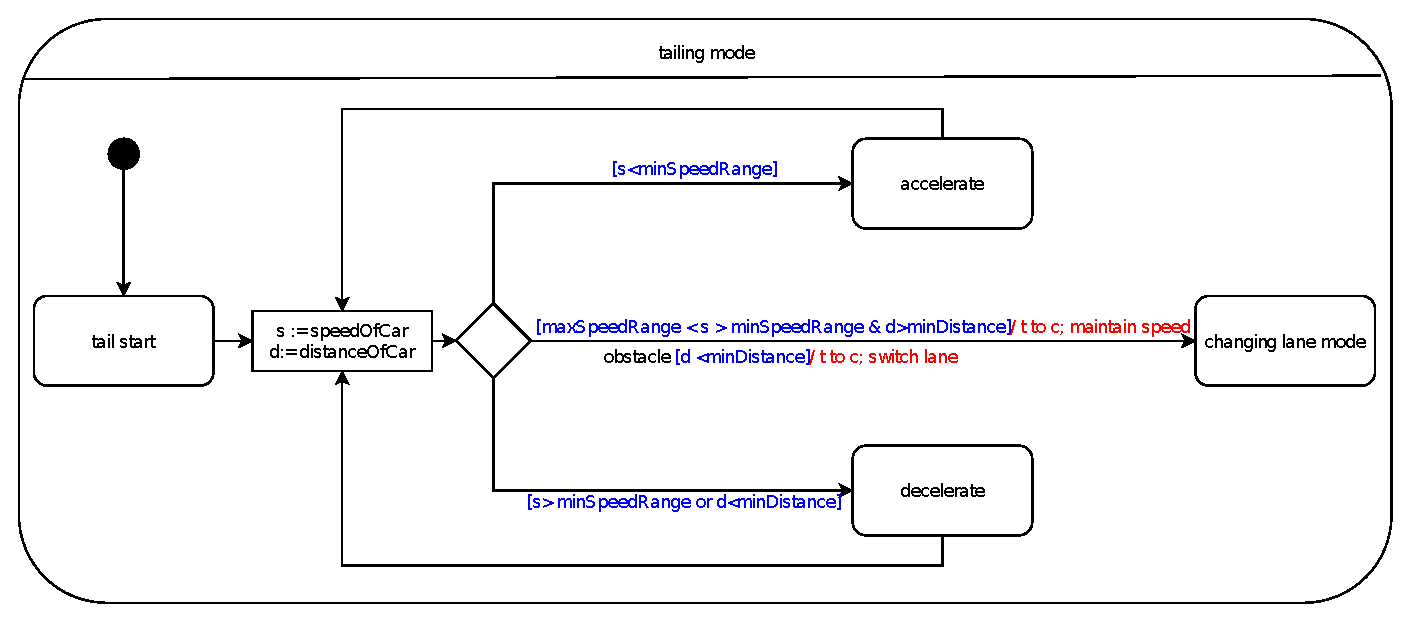
\includegraphics[width=0.8\textwidth]{./A2_Figures/A2_SOEN331_Tailing.eps}
		  \caption{Tailing Mode.}
  \label{fig:tailing-mode-fig}
\end{figure}

\begin{figure}[h!]
	\centering
		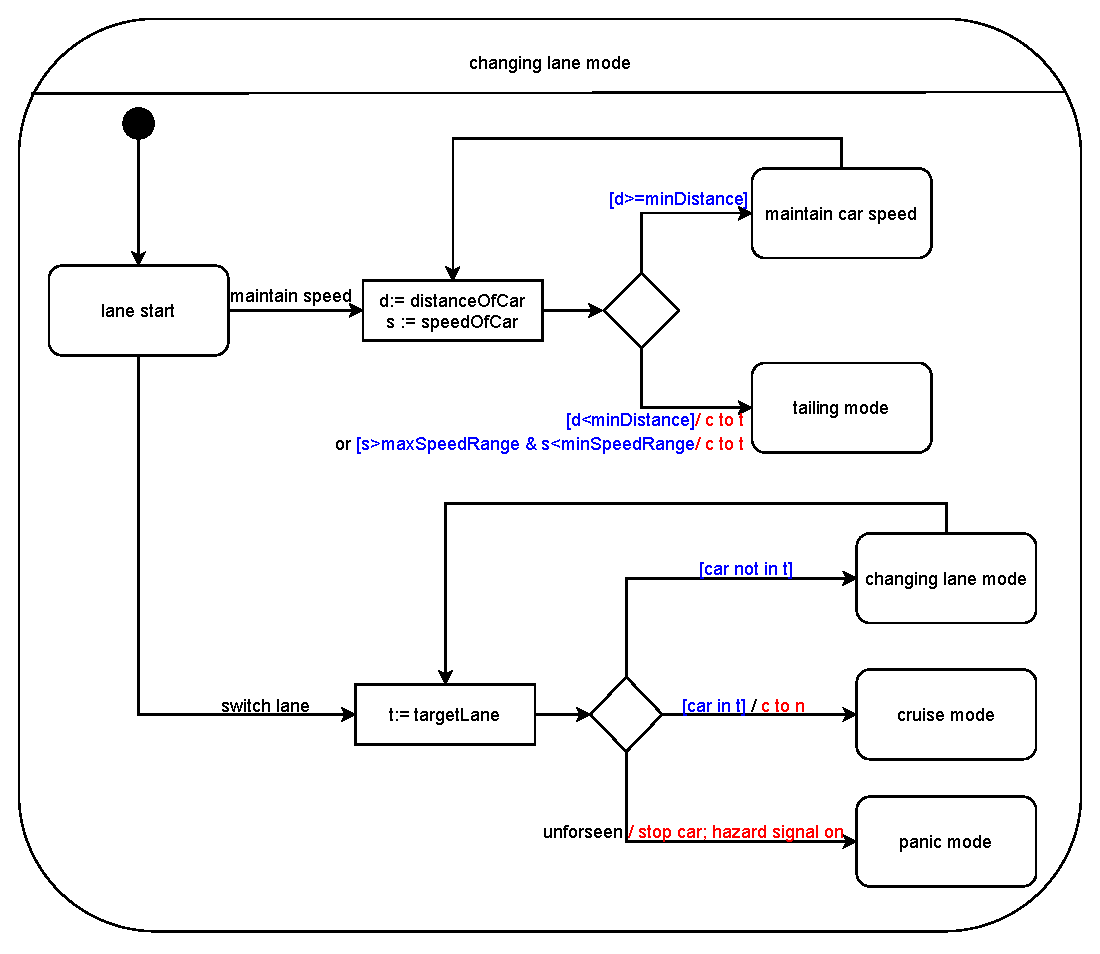
\includegraphics[width=0.8\textwidth]{./A2_Figures/A2_SOEN331_Changing_Lane.eps}
		  \caption{Changing Lane Mode.}
  \label{fig:changing-lane-mode-fig}
\end{figure}

\begin{figure}[h!]
	\centering
		\includegraphics[width=0.8\textwidth]{./A2_Figures/A2_SOEN331_Navigation.eps}
		  \caption{Navigation Mode.}
  \label{fig:navigation-mode-fig}
\end{figure}

\end{spacing}


\end{document}
